

\begin{subsection}{GRMON}
 GRMON is a general debug monitor for the LEON processor, and for SOC designs based on the GRLIB IP
library. GRMON includes the following functions:
\begin{itemize}

 \item Read/write access to all system registers and memory
 \item Built-in disassembler and trace buffer management
 \item Downloading and execution of LEON applications
 \item Breakpoint and watchpoint management
 \item Remote connection to GNU debugger (GDB)
 \item Support for USB, JTAG, RS232, PCI, Ethernet and SpaceWire debug links

\end{itemize}
\end{subsection}
 
\begin{subsection}{ Debug}

The GRMON debug monitor is intended to debug system-on-chip (SOC) designs based on the LEON processor. 
The monitor connects to a dedicated debug interface on the target hardware, through which it can perform
read and write cycles on the on-chip bus (AHB). The debug interface can be of various types: the LEON2 processor
supports debugging over a serial UART and 32-bit PCI, while LEON3 also supports JTAG, ethernet and
spacewire (using the GRESB ethernet to spacewire bridge) debug interfaces. On the target system, all debug
interfaces are realized as AHB masters with the debug protocol implemented in hardware. There is thus no
software support necessary to debug a LEON system, and a target system does in fact not even need to have a
processor present.

 \begin{figure}[ht]
    \centering
    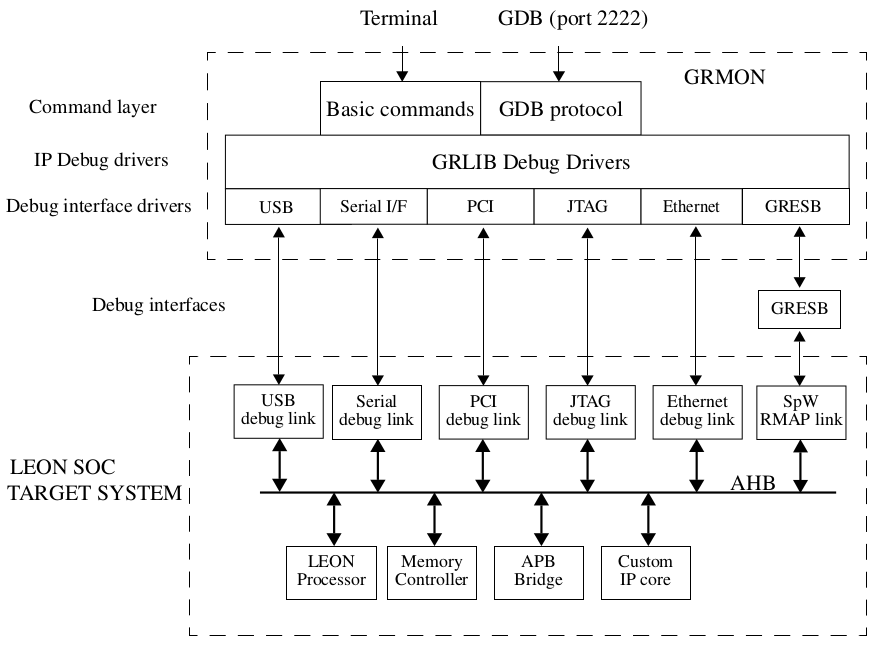
\includegraphics[width=0.75\textwidth]{Figures/others/grmon_ex.png}
    \caption{GRMON  Interface }
    \label{fig:grmon_int}
\end{figure}
GRMON can operate in two modes: command-line mode and GDB mode. In command-line mode, GRMON
commands are entered manually through a terminal window. In GDB mode, GRMON acts as a GDB gateway
and translates the GDB extended-remote protocol to debug commands on the target system.
GRMON is implemented using three functional layers: command layer, debug driver layer, and debug interface
layer. The command layer consist of a general command parser which implements commands that are independent
of the used debug interface or target system. These commands include program downloading and flash
programming.
The debug driver layer implements custom commands which are related to the configuration of the target system. 
GRMON scans the target system at startup, and detects which IP cores are present and how they are con-
figured. For each supported IP core, a debug driver is enabled which implements additional debug commands
for the specific core. Such commands can consist of memory detection routines for memory controllers, or program
debug commands for the LEON processors.
The debug interface layer implements the debug link protocol for each supported debug interface. The protocol
depends on which interface is used, but provides a uniform read/write interface to the upper layers. Which
interface to use for a debug session is specified through command-line options during the start of GRMON.

\end{subsection}

